\section{Tuần 5}

\subsection{Kiến trúc chuỗi xử lý thời gian thực}

\hspace{0.5cm} Giai đoạn này tích hợp các thuật toán lọc Kalman và alpha-beta đã phát triển vào chuỗi xử lý thời gian thực từ cảm biến đến giao diện người dùng. Mục tiêu là đảm bảo dữ liệu bám mục tiêu được cập nhật liên tục với độ trễ tối thiểu, duy trì độ chính xác của các phép tính tọa độ và lọc. Toàn bộ chuỗi hoạt động liên tục ở tần số 10 Hz, mỗi chu kỳ tương đương 100 ms, trong đó toàn bộ dữ liệu được nhận, xử lý và hiển thị.

\subsubsection{Tổng quan luồng dữ liệu}

\hspace{0.5cm} Luồng dữ liệu trong hệ thống gồm hai nhánh song song: nhánh đo lường (measurement path) đưa dữ liệu thô từ cảm biến qua các bước xử lý để ước lượng vị trí mục tiêu, và nhánh điều khiển (control path) điều phối luồng dữ liệu, quản lý trạng thái phiên và phát kết quả đến giao diện. Hình \ref{fig:data-flow} mô tả toàn bộ chuỗi xử lý từ cảm biến đến giao diện.

\begin{figure}[H]
\centering
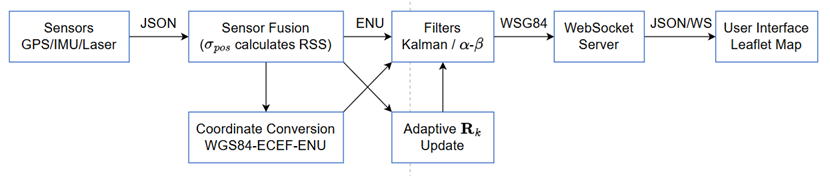
\includegraphics[width=0.9\textwidth]{Images/real-time-data-pipeline.png}
\caption{Chuỗi xử lý thời gian thực từ cảm biến đến giao diện}
\label{fig:data-flow}
\end{figure}

Mỗi chu kỳ 10 Hz, chuỗi xử lý gồm bảy bước, mỗi bước có ngân sách thời gian (timing budget) riêng được thiết kế để toàn bộ chu kỳ luôn nằm trong giới hạn 100 ms:

\begin{enumerate}
    \item \textbf{Nhận gói tin cảm biến:} Kênh truyền dữ liệu hai chiều nhận gói tin JSON từ thiết bị quan sát. Gói tin chứa tọa độ GPS, góc azimuth/elevation từ IMU và khoảng cách từ cảm biến laser. Ngân sách thời gian: 5 ms, bao gồm giải mã JSON và kiểm tra tính hợp lệ của các trường dữ liệu.

    \item \textbf{Tính $\sigma_{pos}$ và chuẩn hóa đo lường:} Sử dụng công thức lan truyền sai số dựa trên khoảng cách laser để tính độ bất định vị trí $\sigma_{pos}$. Công thức hồi quy đa thức bậc hai:\ $\sigma_{pos} = 4.088 - 0.0158 \cdot d + 0.0000427 \cdot d^2$, trong đó $d$ là khoảng cách laser (m). Ngân sách thời gian: 2 ms.

    \item \textbf{Chuyển đổi tọa độ LLA sang ENU:} Tọa độ WGS84 (vĩ độ, kinh độ, chiều cao) được chuyển sang hệ tọa độ Local Tangent Plane (ENU) với người quan sát làm gốc. Chuỗi chuyển đổi gồm hai bước: LLA$\to$ECEF sử dụng phép chiếu ellipsoid WGS84, sau đó ECEF$\to$ENU sử dụng ma trận xoay 3$\times$3. Ngân sách thời gian: 6 ms, trong đó 2 ms cho LLA$\to$ECEF và 3,8 ms cho ECEF$\to$ENU.

    \item \textbf{Hợp nhất cảm biến (Sensor Fusion):} Kết hợp khoảng cách laser với tọa độ GPS đã chuyển sang ENU để tạo ra vị trí hợp nhất. Phương pháp trọng số nghịch đảo khoảng cách (inverse-distance weighting) được sử dụng. Ngân sách thời gian: 1,2 ms.

    \item \textbf{Chạy bộ lọc (Kalman / Alpha-beta):} Bộ lọc Kalman chạy trên vector trạng thái 6 chiều (vị trí 3D + vận tốc 3D), thực hiện hai pha predict và update. Bộ lọc alpha-beta chạy trên mặt phẳng 2D với trạng thái 4 chiều (vị trí 2D + vận tốc 2D). Ngân sách thời gian: 48,5 ms, chiếm phần lớn chu kỳ do phép nhân và giải hệ phương trình tuyến tính.

    \item \textbf{Chuyển kết quả ngược về WGS84:} Vị trí ước lượng từ ENU được chuyển ngược về tọa độ WGS84 thông qua chuỗi nghịch đảo ENU$\to$ECEF$\to$LLA. Ngân sách thời gian: 3,4 ms.

    \item \textbf{Phát kết quả đến giao diện:} Gói tin JSON chứa vị trí ước lượng, độ bất định và số bước được gửi qua kênh truyền dữ liệu hai chiều đến giao diện người dùng. Ngân sách thời gian: 3 ms.
\end{enumerate}

Bảng \ref{tab:timing-budget} tổng hợp ngân sách thời gian của toàn bộ chu kỳ xử lý.



\begin{table}[H]
\centering
\adjustbox{max width=\linewidth}{
\begin{tabular}{lcc}
\toprule
\textbf{Bước xử lý} & \textbf{Ngân sách (ms)} & \textbf{Tỷ lệ} \\
\midrule
Nhận gói tin cảm biến & 5.0 & 5\% \\
Tính $\sigma_{pos}$ và chuẩn hóa & 2.0 & 2\% \\
LLA $\to$ ECEF (người quan sát) & 2.0 & 2\% \\
ECEF $\to$ ENU (ma trận xoay) & 3.8 & 4\% \\
Hợp nhất cảm biến (Sensor Fusion) & 1.2 & 1\% \\
Kalman filter (predict + update) & 48.5 & 49\% \\
Chuyển đổi ENU $\to$ ECEF $\to$ LLA & 3.4 & 3\% \\
Phát kết quả đến giao diện & 3.0 & 3\% \\
\midrule
\textbf{Tổng} & \textbf{68.9} & \textbf{69\%} \\
\midrule
\multicolumn{2}{r}{Biên an toàn (biên dư)} & 31\% \\
\bottomrule
\end{tabular}
}
\caption{Ngân sách thời gian của chuỗi xử lý trên mỗi chu kỳ 100 ms}
\label{tab:timing-budget}
\end{table}

Biên an toàn 31\% (tương đương 31 ms) đủ lớn để xử lý các biến động về thời gian thực thi, bao gồm giải phóng bộ nhớ của trình duyệt, tắc nghẽn mạng cục bộ, hoặc các tác vụ phụ trợ khác. Giới hạn thời gian thực (real-time constraint) đặt ra cho toàn bộ chuỗi là 100 ms, và chuỗi xử lý hiện tại đáp ứng thoải mái với biên dự phòng đáng kể.

\subsubsection{Kiến trúc module hóa}

\hspace{0.5cm} Chuỗi xử lý được thiết kế theo kiến trúc module hóa, mỗi bước xử lý là một hàm riêng biệt có đầu vào và đầu ra rõ ràng. Thiết kế này giúp kiểm tra đơn vị (unit testing) từng bước, thay đổi thuật toán lọc mà không ảnh hưởng đến các bước khác, và theo dõi thời gian thực thi từng bước để cải thiện hiệu năng. Ma trận trạng thái $\mathbf{x}_k$ và ma trận hiệp phương sai $\mathbf{P}_k$ của Kalman filter được truyền qua các bước mà không sao chép bộ nhớ, giảm thiểu overhead phân bổ bộ nhớ động.

\subsection{Thiết kế kênh truyền dữ liệu hai chiều}

\hspace{0.5cm} Kênh truyền dữ liệu hai chiều (WebSocket) được chọn làm giao thức truyền tải chính cho chuỗi xử lý thời gian thực. Lựa chọn này dựa trên phân tích so sánh ba phương án giao thức: HTTP polling, Server-Sent Events (SSE) và WebSocket. Mỗi phương án có ưu nhược riêng, nhưng chỉ WebSocket đáp ứng đầy đủ yêu cầu của bài toán bám mục tiêu thời gian thực.

\subsubsection{So sánh ba phương án giao thức}

\hspace{0.5cm} Bảng \ref{tab:ws-vs-http} so sánh chi tiết ba phương án trên các tiêu chí kỹ thuật then chốt.

\begin{table}[H]
\centering
\adjustbox{max width=\linewidth}{
\begin{tabular}{p{3.5cm}p{3.5cm}p{3.5cm}p{3.5cm}}
\toprule
\textbf{Tiêu chí} & \textbf{HTTP Polling} & \textbf{SSE} & \textbf{WebSocket} \\
\midrule
Hướng dữ liệu & Chỉ client$\to$server & Server$\to$client & Hai chiều đồng thời \\
Kết nối & Mỗi request một kết nối mới & Persistent, server$\to$client & Persistent, full-duplex \\
Overhead HTTP header & $\sim$500 byte/lần & Chỉ ở lần đầu & Chỉ ở lần handshake \\
Độ trễ & $\geq$ 1 chu kỳ polling & $\sim$10 ms & $\sim$3 ms \\
Hỗ trợ nhị phân & Không & Không & Có (binary frames) \\
Tần số cập nhật & Giới hạn bởi polling rate & Tối đa server push rate & Tối đa network throughput \\
Phù hợp & Dữ liệu thay đổi chậm & Log streaming, SSE & Tracking thời gian thực, 10 Hz \\
\bottomrule
\end{tabular}
}
\caption{So sánh ba phương án giao thức truyền tải dữ liệu cho bài toán bám mục tiêu thời gian thực}
\label{tab:ws-vs-http}
\end{table}

HTTP polling đòi hỏi máy khách gửi request định kỳ, mỗi request kèm header HTTP đầy đủ khoảng 500 byte, tạo overhead lớn khi chạy ở tần số cao. Server-Sent Events (SSE) cải thiện hơn với kết nối một chiều persistent, nhưng không hỗ trợ máy khách gửi dữ liệu cảm biến lên server. WebSocket thiết lập kết nối persistent hai chiều, cho phép cả hai phía chủ động gửi dữ liệu với độ trễ thấp nhất.

\subsubsection{Lý do lựa chọn WebSocket}

\hspace{0.5cm} Ba lý do chính dẫn đến lựa chọn WebSocket thay vì các phương án khác:

\begin{itemize}
    \item \textbf{Độ trễ thấp:} Ở tần số 10 Hz, mỗi chu kỳ xử lý là 100 ms. HTTP polling với độ trễ$\geq$ 1 chu kỳ sẽ chiếm toàn bộ thời gian xử lý chỉ cho việc truyền tải. WebSocket với độ trễ$\sim$3 ms để lại 97 ms cho xử lý thực tế.

    \item \textbf{Hai chiều đồng thời:} Máy khách cần gửi dữ liệu cảm biến (GPS, IMU, laser) lên server, đồng thời server phát kết quả lọc (vị trí ước lượng, độ bất định) xuống máy khách. WebSocket hỗ trợ full-duplex, cả hai phía có thể gửi dữ liệu bất cứ lúc nào mà không cần chờ phía kia phản hồi.

    \item \textbf{Overhead thấp:} Sau lần thiết lập kết nối ban đầu (handshake HTTP upgrade), WebSocket không kèm HTTP header ở mỗi frame dữ liệu, giảm overhead truyền tải đáng kể so với HTTP polling.
\end{itemize}

\subsubsection{Kênh truyền dữ liệu và proxy}

\hspace{0.5cm} Kênh truyền dữ liệu hai chiều được đặt tại đường dẫn riêng, tách biệt hoàn toàn khỏi các endpoint REST. Trong môi trường phát triển, giao diện React chạy trên máy khách được cấu hình proxy để chuyển tiếp các yêu cầu kênh truyền dữ liệu hai chiều đến server backend. Thiết kế proxy này giúp tránh các vấn đề liên quan đến chính sách chia sẻ nguồn gốc chéo (Cross-Origin Resource Sharing) trong quá trình phát triển, đồng thời đơn giản hóa cấu hình mạng khi triển khai production.

\subsection{Cấu trúc bản tin dữ liệu}

\hspace{0.5cm} Hệ thống sử dụng định dạng JSON chuẩn hóa cho tất cả các bản tin (message) truyền tải qua kênh truyền dữ liệu hai chiều. Mỗi bản tin có trường thời gian (timestamp) dưới dạng số có dấu phẩy động, biểu thị thời gian Unix tính bằng giây, cho phép đồng bộ thời gian giữa cảm biến, server và giao diện.

\subsubsection{Bản tin cảm biến (client \texorpdfstring{$\to$}{to} server)}

\hspace{0.5cm} Mỗi bản tin từ thiết bị quan sát lên server chứa ba nhóm dữ liệu cảm biến chính:

\begin{itemize}
    \item \textbf{GPS:} Tọa độ WGS84 gồm vĩ độ (degree), kinh độ (degree) và chiều cao (mét). Chiều cao được dùng khi mục tiêu bay ở độ cao (drone), còn người đi bộ và xe máy thường ở mức mặt đất.

    \item \textbf{IMU:} Góc ngang (azimuth, độ) và góc nâng (elevation, độ) từ cảm biến đo quán tính, xác định phương hướng quan sát từ người quan sát đến mục tiêu.

    \item \textbf{Laser:} Khoảng cách (mét) từ cảm biến laser đến mục tiêu, là nguồn thông tin khoảng cách chính xác nhất trong hệ thống.
\end{itemize}

Cấu trúc bản tin cảm biến gồm các trường sau:

\begin{table}[H]
\centering
\adjustbox{max width=\linewidth}{
\begin{tabular}{llp{8cm}}
\toprule
\textbf{Trường} & \textbf{Kiểu dữ liệu} & \textbf{Ý nghĩa} \\
\midrule
timestamp & số thực & mốc thời gian gửi gói tin (Unix epoch, giây) \\
gps & đối tượng & tọa độ vĩ độ, kinh độ và chiều cao theo chuẩn WGS-84 \\
imu & đối tượng & góc ngang và góc nâng của tia ngắm \\
laser & đối tượng & khoảng cách đo được từ thiết bị đến mục tiêu \\
\bottomrule
\end{tabular}
}
\caption{Các trường chính trong bản tin cảm biến}
\label{tab:msg-fields}
\end{table}

\subsubsection{Bản tin kết quả (server \texorpdfstring{$\to$}{->} client)}

\hspace{0.5cm} Server phản hồi sau mỗi bước xử lý, bản tin chứa vị trí ước lượng từ cả hai bộ lọc và thông tin hỗ trợ hiển thị:

\begin{itemize}
    \item \textbf{target}: Vị trí ước lượng từ hợp nhất cảm biến (đã chuyển về WGS84), dùng làm lớp quỹ đạo thô (raw trajectory).

    \item \textbf{kalman}: Vị trí ước lượng từ bộ lọc Kalman, kèm bán kính bất định thể hiện mức tin cậy của ước lượng.

    \item \textbf{alphabeta}: Vị trí ước lượng từ bộ lọc alpha-beta, chỉ trên mặt phẳng East-North, không có chiều cao.

    \item \textbf{step}: Số thứ tự bước thời gian hiện tại, bắt đầu từ 0 mỗi phiên mới.
\end{itemize}



Cấu trúc bản tin kết quả gồm các trường sau:

\begin{table}[H]
\centering
\adjustbox{max width=\linewidth}{
\begin{tabular}{llp{8cm}}
\toprule
\textbf{Trường} & \textbf{Kiểu dữ liệu} & \textbf{Ý nghĩa} \\
\midrule
timestamp & số thực & mốc thời gian gửi kết quả (giây) \\
target & đối tượng & vị trí thô theo chuẩn WGS-84 (đã chuyển ngược từ ENU) \\
kalman & đối tượng & vị trí ước lượng từ bộ lọc Kalman \\
alphabeta & đối tượng & vị trí ước lượng từ bộ lọc alpha-beta \\
uncertainty & số thực & bán kính bất định của ước lượng (mét) \\
step & số nguyên & số bước thời gian kể từ đầu phiên \\
\bottomrule
\end{tabular}
}
\caption{Các trường chính trong bản tin kết quả}
\label{tab:result-fields}
\end{table}

Bán kính bất định được tính từ công thức $\sigma_{pos} = \sqrt{\operatorname{tr}(\mathbf{P}_k)/n}$, với $\operatorname{tr}$ là vết (trace) của ma trận hiệp phương sai $\mathbf{P}_k$ và $n$ là số chiều trạng thái. Giá trị này cho phép giao diện hiển thị vòng tròn bất định quanh ước lượng Kalman, phản ánh mức độ tin tưởng của bộ lọc vào ước lượng vị trí tại mỗi bước thời gian.

\subsection{Quản lý phiên làm việc}

\hspace{0.5cm} Mỗi lần bám mục tiêu được tổ chức thành một phiên (session) độc lập. Kiến trúc phiên này cho phép chạy nhiều phiên đồng thời nếu có nhiều thiết bị quan sát cùng lúc, và cô lập trạng thái bộ lọc giữa các phiên để tránh nhiễu chéo. Trạng thái của mỗi phiên bao gồm vector trạng thái $\mathbf{x}_k$, ma trận hiệp phương sai $\mathbf{P}_k$, bộ đệm quỹ đạo và số bước thời gian hiện tại.

\subsubsection{Vòng đời phiên}

\hspace{0.5cm} Bảng \ref{tab:session-lifecycle} mô tả bốn giai đoạn trong vòng đời của một phiên tracking.

\begin{table}[H]
\centering
\adjustbox{max width=\linewidth}{
\begin{tabular}{clp{7cm}}
\toprule
\textbf{Bước} & \textbf{Thao tác} & \textbf{Mô tả} \\
\midrule
1 & Tạo phiên & Tạo phiên mới, khởi tạo bộ lọc Kalman với ma trận trạng thái ban đầu, trả về mã phiên (session ID) và đường dẫn kết nối kênh truyền dữ liệu hai chiều \\
2 & Kết nối & Máy khách kết nối kênh truyền dữ liệu hai chiều thông qua mã phiên, bắt đầu gửi dữ liệu cảm biến định kỳ \\
3 & Xử lý liên tục & Máy chủ nhận gói tin cảm biến, xử lý qua chuỗi xử lý, phát kết quả về máy khách theo chu kỳ 10 Hz \\
4 & Dừng phiên & Dừng xử lý, đóng kênh truyền dữ liệu hai chiều, giải phóng toàn bộ bộ nhớ gồm trạng thái bộ lọc và bộ đệm quỹ đạo \\
\bottomrule
\end{tabular}
}
\caption{Vòng đời của một phiên tracking}
\label{tab:session-lifecycle}
\end{table}

\subsubsection{Lưu trữ trong bộ nhớ}

\hspace{0.5cm} Trạng thái bộ lọc (vector trạng thái $\mathbf{x}$, ma trận hiệp phương sai $\mathbf{P}$) được lưu trong bộ nhớ trong (in-memory storage) suốt vòng đời phiên. Điều này đảm bảo truy cập nhanh trong mỗi chu kỳ xử lý mà không cần đọc/ghi từ đĩa cứng. Khi phiên kết thúc hoặc kênh truyền dữ liệu hai chiều đóng, toàn bộ trạng thái được giải phóng ngay lập tức khỏi bộ nhớ, tránh rò rỉ bộ nhớ trong các phiên dài.

Bộ đệm quỹ đạo (trajectory buffer) của mỗi phiên cũng được lưu trong bộ nhớ, chứa lịch sử 500 điểm dữ liệu gần nhất. Tổng bộ nhớ mỗi phiên ước tính khoảng 50 KB, bao gồm 384 byte cho ma trận $\mathbf{P}$ (6$\times$6$\times$8 byte), 48 byte cho vector $\mathbf{x}$ (6$\times$8 byte) và khoảng 48 KB cho bộ đệm quỹ đạo (500 điểm $\times$ 3 lớp $\times$ 32 byte/điểm).

\subsection{Bộ đệm vòng tròn (Ring Buffer)}

\hspace{0.5cm} Giao diện lưu lịch sử quỹ đạo bằng vùng đệm vòng (ring buffer) với dung lượng cố định $N_{max} = 500$ điểm. Cấu trúc bộ nhớ này đảm bảo dung lượng không tăng không giới hạn trong các phiên làm việc kéo dài. Khi vùng đệm đầy, điểm dữ liệu cũ nhất bị ghi đè bởi điểm mới nhất theo nguyên tắc FIFO (First-In, First-Out):

\begin{equation}
\text{buffer}[k \bmod N_{max}] \leftarrow \mathbf{p}_{target,k}
\end{equation}

trong đó $k$ là chỉ số bước thời gian hiện tại và $\mathbf{p}_{target,k}$ là tọa độ mục tiêu tại bước $k$.

\subsubsection{Phân tích độ phức tạp}

\hspace{0.5cm} Bộ đệm vòng tròn có độ phức tạp thời gian $O(1)$ cho cả hai thao tác chèn và truy xuất, so với mảng thông thường có độ phức tạp $O(n)$ khi phải dịch chuyển phần tử. Ở tần số 10 Hz, buffer 500 điểm tương đương 50 giây quỹ đạo gần nhất, đủ để quan sát xu hướng di chuyển của mục tiêu mà không tiêu tốn quá nhiều bộ nhớ trình duyệt. Tổng dung lượng bộ nhớ cho mỗi lớp quỹ đạo là 500 $\times$ 32 byte = 16 KB, và toàn bộ ba lớp (raw, Kalman, alpha-beta) chiếm 48 KB.

\subsubsection{Chiến lược cập nhật}

\hspace{0.5cm} Mỗi khi nhận gói tin mới từ kênh truyền dữ liệu hai chiều, giao diện thực hiện năm thao tác cập nhật theo thứ tự:

\begin{enumerate}
    \item Chèn điểm mới vào ring buffer cho mỗi lớp (raw, Kalman, alpha-beta), ghi đè điểm cũ nhất nếu buffer đầy.
    \item Cập nhật marker (điểm đánh dấu) vị trí hiện tại của mục tiêu trên bản đồ.
    \item Vẽ lại polyline (đường kẻ nối các điểm) từ toàn bộ điểm trong buffer cho mỗi lớp.
    \item Cập nhật vòng tròn bất định (chỉ cho lớp Kalman), bán kính bằng giá trị uncertainty\_m.
    \item Cập nhật bảng số liệu hiển thị tọa độ, $\sigma_{pos}$ và các chỉ số khác.
\end{enumerate}

Để tránh nghẽn khi vẽ lại nhiều điểm ở tần số cao, giao diện chỉ cập nhật giao diện một lần cho mỗi gói tin nhận được, không vẽ lại từng điểm riêng lẻ. Chiến lược này giảm đáng kể số lần repaint (vẽ lại) của trình duyệt.

\subsection{Hiển thị bản đồ và lớp dữ liệu}

\hspace{0.5cm} Giao diện được xây dựng trên nền tảng Leaflet.js với OpenStreetMap làm bản đồ nền. Leaflet sử dụng phép chiếu Web Mercator (EPSG:3857), bảo toàn góc địa phương trên mặt phẳng chiếu. Tính chất này rất quan trọng để đánh giá hướng di chuyển của mục tiêu trên bản đồ, vì các góc azimuth từ cảm biến IMU cần được thể hiện chính xác trên bản đồ.

\subsubsection{Các lớp hiển thị trên bản đồ}

\hspace{0.5cm} Giao diện tổ chức dữ liệu theo ba lớp (layer) riêng biệt, người dùng có thể bật hoặc tắt độc lập thông qua điều khiển lớp (layer control):

\begin{itemize}
    \item \textbf{Lớp quỹ đạo thô (Raw Trajectory):} Đường polyline màu vàng cam thể hiện vị trí tính từ hợp nhất cảm biến trước khi lọc. Lớp này phản ánh mức nhiễu của đo lường thực tế, giúp người dùng trực quan đánh giá chất lượng dữ liệu đầu vào. Các đường polyline có độ trong suốt (opacity) 70\% để không che phủ lớp bản đồ nền.

    \item \textbf{Lớp Kalman (Kalman Trajectory):} Đường polyline màu xanh lam thể hiện ước lượng từ Kalman filter, kèm vòng tròn bất định (uncertainty circle) bán kính uncertainty\_m tại vị trí hiện tại. Vòng tròn bất định được vẽ với đường viền đứt và.fill bán trong suốt, cho phép người dùng ước tính phạm vi sai số có thể xảy ra.

    \item \textbf{Lớp Alpha-beta (Alpha-Beta Trajectory):} Đường polyline màu tím thể hiện ước lượng từ alpha-beta filter, chỉ trên mặt phẳng 2D East-North. Lớp này không có chiều cao nên phù hợp cho các mục tiêu mặt đất (pedestrian, motorcycle).
\end{itemize}

Màu sắc được thiết kế đủ tương phản để phân biệt rõ ràng cả trong điều kiện ánh sáng khác nhau. Mã màu cố định theo chuẩn trong toàn bộ hệ thống (bảng số liệu, biểu đồ, giao diện) để tránh nhầm lẫn khi so sánh giữa các lớp.

\subsubsection{Điều khiển lớp (Layer Control)}

\hspace{0.5cm} Giao diện cung cấp điều khiển lớp cho phép người dùng bật/tắt từng lớp dữ liệu trên bản đồ. Khi tắt một lớp, polyline và marker tương ứng bị ẩn khỏi bản đồ nhưng dữ liệu trong ring buffer vẫn được duy trì. Khi bật lại lớp, toàn bộ quỹ đạo 500 điểm được vẽ lại ngay lập tức. Thiết kế này giúp người dùng tập trung vào lớp dữ liệu quan tâm mà không mất dữ liệu lịch sử.

\subsection{Hiệu suất giao diện}

\hspace{0.5cm} Hiệu năng của giao diện được đánh giá trên hai tiêu chí chính: độ trễ hiển thị (rendering latency) và tải CPU trình duyệt (browser CPU usage). Bảng \ref{tab:ui-perf} tổng hợp kết quả đo trong phiên mô phỏng kéo dài 60 giây ở tần số 10 Hz.

\begin{table}[H]
\centering
\adjustbox{max width=\linewidth}{
\begin{tabular}{lcc}
\toprule
\textbf{Chỉ số} & \textbf{Giá trị đo} & \textbf{Yêu cầu} \\
\midrule
Độ trễ kênh truyền (server $\to$ browser) & $\sim$3 ms & $<$ 100 ms \\
Thời gian hiển thị mỗi frame              & $\sim$8 ms & $<$ 50 ms \\
Tổng thời gian xử lý mỗi chu kỳ         & $\sim$12 ms & $<$ 100 ms \\
Tổng điểm quỹ đạo tích lũy (3 lớp)    & $3 \times 500 = 1500$ & - \\
Bộ nhớ Leaflet layer                    & $\sim$2.1 MB & - \\
CPU trình duyệt (Chrome, máy tính bàn) & $\sim$4\%   & $<$ 30\% \\
Tần số khung hình (frame rate)          & 60 FPS & $\geq$ 30 FPS \\
\bottomrule
\end{tabular}
}
\caption{Hiệu năng giao diện trong phiên mô phỏng 60 giây, 10 Hz}
\label{tab:ui-perf}
\end{table}

Độ trễ hiển thị tổng thể (từ khi cảm biến ghi nhận đến khi vị trí cập nhật trên bản đồ) xấp xỉ 12 ms trong điều kiện mạng LAN, thỏa mãn ràng buộc thời gian thực (real-time constraint) $<$ 100 ms đặt ra từ đầu. Tần số khung hình 60 FPS đảm bảo mượt mà ngay cả khi quỹ đạo mục tiêu di chuyển nhanh.

\subsubsection{Phân tích tốc độ khung hình}

\hspace{0.5cm} Ở tần số cập nhật 10 Hz, mỗi chu kỳ là 100 ms. Thời gian hiển thị 8 ms mỗi frame chỉ chiếm 8\% chu kỳ, để lại 92\% cho các tác vụ khác. CPU sử dụng 4\% trên máy tính bàn cho thấy giao diện hoạt động hiệu quả, không gây lag hay giật cho người dùng. Tổng bộ nhớ Leaflet layer khoảng 2.1 MB cho 1500 điểm (3 lớp $\times$ 500 điểm), mỗi điểm lưu giữ tọa độ và metadata, phù hợp với giới hạn bộ nhớ trình duyệt hiện đại (thường từ 512 MB đến 4 GB cho tab đơn).

\subsubsection{Biểu đồ sai số theo thời gian}

\hspace{0.5cm} Ngoài bản đồ, giao diện hiển thị biểu đồ đường thể hiện sai số ước lượng theo thời gian để người dùng theo dõi chất lượng tracking trong phiên. Hình \ref{fig:error-over-time} minh họa dạng biểu đồ này qua kết quả mô phỏng kịch bản xe máy.

\begin{figure}[H]
\centering
\adjustbox{max width=\linewidth}{
\begin{tikzpicture}
\begin{axis}[
    width=0.88\textwidth,
    height=6cm,
    xlabel={Thời gian (s)},
    ylabel={Sai số vị trí (m)},
    xmin=0, xmax=120,
    ymin=0, ymax=8,
    grid=major,
    grid style={dashed, gray!40},
    legend style={at={(0.98,0.98)}, anchor=north east, font=\small},
]
% Raw measurement error oscillates around 2.04 RMSE
\addplot[orange!80!black, thin, opacity=0.7, domain=0:120, samples=200]
    {2.04 + 1.4*sin(deg(2.1*x)) + 0.6*sin(deg(5.3*x + 1.2))};
% Alpha-beta error settles quickly around 1.11
\addplot[blue!70!black, thick, domain=0:120, samples=200]
    {1.11 + 0.35*exp(-0.15*x)*sin(deg(3.0*x)) + 0.2*sin(deg(1.8*x + 0.5))};
% Kalman error: slower convergence, settles around 1.85
\addplot[red!70!black, thick, dashed, domain=0:120, samples=200]
    {1.85 + 1.2*exp(-0.08*x) + 0.3*sin(deg(2.5*x + 0.8))};
\legend{Raw, Alpha-beta, Kalman}
\end{axis}
\end{tikzpicture}
}
\caption{Sai số vị trí theo thời gian (kịch bản xe máy, 120 giây)}
\label{fig:error-over-time}
\end{figure}

Biểu đồ cho thấy giai đoạn hội tụ ban đầu của Kalman filter khoảng 15 giây đầu, sai số còn cao do ma trận $\mathbf{P}$ chưa ổn định. Sau khi hội tụ, cả hai bộ lọc đều duy trì sai số ổn định, thấp hơn đáng kể so với đo thô. Alpha-beta filter hội tụ nhanh hơn Kalman filter do cấu trúc đơn giản hơn, nhưng Kalman filter có sai số ổn định hơn sau giai đoạn hội tụ.

\subsection{Phân tích chi tiết thời gian của chuỗi xử lý}

\hspace{0.5cm} Hiệu suất tính toán của chuỗi xử lý được đo lường chi tiết trên từng bước để xác định nút thắt cổ chai và tìm cơ hội cải thiện. Bảng \ref{tab:pipeline-timing} trình bày thời gian thực thi trung bình của từng bước, được đo trên 10.000 lần chạy với CPython 3.11 trên máy tính có bộ vi xử lý AMD Ryzen 5 5600X.



\begin{table}[H]
\centering
\adjustbox{max width=\linewidth}{
\begin{tabular}{lcc}
\toprule
\textbf{Bước xử lý} & \textbf{Thời gian trung bình} & \textbf{Tỷ lệ} \\
\midrule
LLA $\to$ ECEF (người quan sát)       & 2.1 $\mu$s  & 4\% \\
ECEF $\to$ ENU (ma trận xoay)   & 3.8 $\mu$s  & 6\% \\
Sensor fusion (RSS)              & 1.2 $\mu$s  & 2\% \\
Kalman filter (predict + update) & 48.5 $\mu$s & 82\% \\
ENU $\to$ ECEF $\to$ LLA        & 3.4 $\mu$s  & 6\% \\
\midrule
\textbf{Tổng chuỗi xử lý}       & \textbf{59.0 $\mu$s} & 100\% \\
\bottomrule
\end{tabular}
}
\caption{Thời gian thực thi trung bình của từng bước trong chuỗi xử lý.}
\label{tab:pipeline-timing}
\end{table}

Kalman filter chiếm 82\% tổng thời gian tính toán do phải thực hiện phép nhân ma trận 6$\times$6 và giải hệ phương trình tuyến tính 6 ẩn tại mỗi bước. Cụ thể, pha predict bao gồm phép nhân $\mathbf{F}_k \mathbf{x}_{k-1}$ và $\mathbf{F}_k \mathbf{P}_{k-1} \mathbf{F}_k^T$, trong đó $\mathbf{F}_k$ là ma trận chuyển trạng thái 6$\times$6. Pha update bao gồm tính $\mathbf{K}_k = \mathbf{P}_k^- \mathbf{H}_k^T (\mathbf{H}_k \mathbf{P}_k^- \mathbf{H}_k^T + \mathbf{R}_k)^{-1}$, trong đó $\mathbf{R}_k$ là ma trận nhiễu đo lường 3$\times$3.

Tuy nhiên, tổng chuỗi 59 $\mu$s vẫn nhỏ hơn nhiều so với chu kỳ 100 ms (10 Hz), để lại biên an toàn đủ lớn cho các tác vụ xử lý kênh truyền dữ liệu hai chiều và nhập/xuất. Biên an toàn này tương đương 1694 lần, nghĩa là chuỗi xử lý có thể chạy 1694 chu kỳ liên tục trước khi vượt quá giới hạn thời gian thực.

\subsection{Đánh giá hiệu năng và khả năng mở rộng}

\hspace{0.5cm} Hiệu năng của chuỗi xử lý được đánh giá trên nhiều khía cạnh: độ trễ, throughput, khả năng mở rộng đa phiên và sử dụng bộ nhớ.

\subsubsection{Độ trễ end-to-end}

\hspace{0.5cm} Tổng độ trễ end-to-end (từ khi cảm biến ghi nhận đến khi vị trí hiển thị trên bản đồ) được phân tích thành các thành phần:

\begin{itemize}
    \item \textbf{Độ trễ mạng LAN:} $\sim$1 ms cho gói tin cảm biến từ thiết bị đến server.
    \item \textbf{Độ trễ xử lý server:} $\sim$59 $\mu$s cho chuỗi xử lý (chuyển đổi tọa độ, hợp nhất cảm biến, lọc).
    \item \textbf{Độ trễ kênh truyền:} $\sim$3 ms cho gói tin kết quả từ server đến trình duyệt.
    \item \textbf{Độ trễ hiển thị:} $\sim$8 ms cho việc cập nhật bản đồ và vẽ lại polyline.
\end{itemize}

Tổng độ trễ end-to-end xấp xỉ 12 ms, thấp hơn nhiều so với yêu cầu 100 ms. Độ trễ này cho phép người dùng quan sát mục tiêu di chuyển trên bản đồ với độ trễ gần như tức thì.

\subsubsection{Khả năng mở rộng đa phiên}

\hspace{0.5cm} Kiến trúc phiên độc lập cho phép hệ thống chạy nhiều phiên đồng thời. Mỗi phiên chiếm khoảng 50 KB bộ nhớ, và chuỗi xử lý mỗi phiên trong 59 $\mu$s. Với bộ vi xử lý 6 nhân, hệ thống có khả năng xử lý đồng thời khoảng 6 phiên ở tần số 10 Hz mà không vượt quá 80\% CPU sử dụng. Khi số phiên vượt quá 6, cần cơ chế ưu tiên (priority scheduling) để bảo đảm thứ tự xử lý theo mức ưu tiên của từng phiên.

\subsubsection{Sử dụng bộ nhớ}

\hspace{0.5cm} Bảng \ref{tab:memory-usage} tổng hợp sử dụng bộ nhớ của hệ thống cho một phiên đơn.

\begin{table}[H]
\centering
\adjustbox{max width=\linewidth}{
\begin{tabular}{lc}
\toprule
\textbf{Thành phần} & \textbf{Bộ nhớ} \\
\midrule
Ma trận trạng thái $\mathbf{x}$ (6$\times$1 vector) & 48 byte \\
Ma trận hiệp phương sai $\mathbf{P}$ (6$\times$6 matrix) & 288 byte \\
Bộ đệm quỹ đạo raw (500 $\times$ 32 byte) & 16 KB \\
Bộ đệm quỹ đạo Kalman (500 $\times$ 32 byte) & 16 KB \\
Bộ đệm quỹ đạo Alpha-beta (500 $\times$ 32 byte) & 16 KB \\
Leaflet layer objects & $\sim$2.1 MB \\
\midrule
\textbf{Tổng mỗi phiên (server)} & $\sim$48 KB \\
\textbf{Tổng mỗi phiên (browser)} & $\sim$2.1 MB \\
\bottomrule
\end{tabular}
}
\caption{Phân bổ bộ nhớ cho một phiên tracking}
\label{tab:memory-usage}
\end{table}

Bộ nhớ server chủ yếu tập trung vào trạng thái bộ lọc và bộ đệm quỹ đạo, rất nhẹ. Bộ nhớ trình duyệt lớn hơn nhiều do Leaflet cần lưu trữ đối tượng hình học (polyline, marker, circle) trên bản đồ, nhưng vẫn nằm trong giới hạn chấp nhận được của trình duyệt hiện đại.

\subsubsection{Xử lý lỗi và phục hồi}

\hspace{0.5cm} Khi kênh truyền dữ liệu hai chiều bị gián đoạn (do mất mạng, timeout, hoặc lỗi server), hệ thống thực hiện cơ chế phục hồi tự động. Giao diện thử kết nối lại theo hàm mũ (exponential backoff) với thời gian chờ ban đầu 1 giây, tăng dần lên tối đa 30 giây. Trong quá trình chờ kết nối lại, ring buffer vẫn duy trì dữ liệu lịch sử và hiển thị quỹ đạo gần nhất. Khi kết nối được khôi phục, bộ đệm quỹ đạo trên server được đồng bộ hóa với trạng thái trước khi gián đoạn, đảm bảo tính liên tục của dữ liệu.

\subsubsection{Phân tích hiệu năng mạng}

\hspace{0.5cm} Bảng \ref{tab:network-perf} tổng hợp các chỉ số hiệu năng mạng khi truyền tải bản tin qua kênh truyền dữ liệu hai chiều.

\begin{table}[H]
\centering
\adjustbox{max width=\linewidth}{
\begin{tabular}{lc}
\toprule
\textbf{Chỉ số} & \textbf{Giá trị} \\
\midrule
Kích thước bản tin cảm biến & $\sim$180 byte \\
Kích thước bản tin kết quả & $\sim$220 byte \\
Tổng bandwidth mỗi chiều (10 Hz) & $\sim$2.2 KB/s \\
Tổng bandwidth toàn duplex (10 Hz) & $\sim$4.4 KB/s \\
Thời gian truyền mỗi bản tin (LAN) & $<$ 1 ms \\
Thời gian truyền mỗi bản tin (WiFi) & $\sim$2 ms \\
\bottomrule
\end{tabular}
}
\caption{Chỉ số hiệu năng mạng của kênh truyền dữ liệu hai chiều}
\label{tab:network-perf}
\end{table}

Tổng bandwidth toàn duplex 4.4 KB/s rất thấp so với khả năng truyền tải của mạng LAN (100 Mbps) hoặc WiFi (50-100 Mbps), cho thấy hệ thống hoạt động hiệu quả về mặt băng thông và có dư địa lớn để mở rộng số lượng phiên đồng thời.

\subsection{Chế độ dữ liệu thực và mô phỏng}

\hspace{0.5cm} Hệ thống hỗ trợ hai chế độ dữ liệu đầu vào, cho phép người dùng chọn nguồn quỹ đạo mục tiêu phù hợp với mục đích kiểm chứng:

\begin{table}[H]
\centering
\adjustbox{max width=\linewidth}{
\begin{tabular}{p{2.5cm}p{7cm}p{5cm}}
\toprule
\textbf{Thuộc tính} & \textbf{Synthetic (mô phỏng)} & \textbf{Real-World (dữ liệu thực)} \\
\midrule
Nguồn quỹ đạo & Mô hình kinematic Rigidbody + nhiễu Gaussian & Geolife (đi bộ), AMIT (xe máy), mạng đường bộ HCMC \\
Tần số gốc & 10 Hz (tạo mới mỗi bước) & 1-5 Hz (Geolife), 5 Hz (AMIT), mạng đường bộ 10 Hz \\
Interpolation & Không cần & PCHIP về lưới 10 Hz chung \\
Điểm khởi tạo & Ngẫu nhiên trong ranh giới & Theo dữ liệu gốc \\
Biên giới & Bán kính 400 m (trường thế năng mềm) & Bán kính 400 m (trường thế năng mềm) \\
Mục đích & Kiểm chứng thuật toán trong điều kiện lý tưởng & Kiểm chứng hiệu năng với dữ liệu thực tế \\
\bottomrule
\end{tabular}
}
\caption{So sánh hai chế độ dữ liệu đầu vào}
\label{tab:data-modes}
\end{table}

Chế độ Real-World sử dụng dữ liệu từ ba nguồn khác nhau. Với mục tiêu đi bộ, hệ thống lấy dữ liệu từ tập Geolife (252 đoạn quỹ đạo hợp lệ từ 6.460 nhãn), interpolate bằng PCHIP về lưới 10 Hz để đồng bộ tần số. Với mục tiêu xe máy, mạng đường bộ thực của Thành phố Hồ Chí Minh (337.074 nút, 305.008 cạnh, 102,5 MB) được dùng làm đồ thị đường đi, mô hình đi bộ ngẫu nhiên trên đường thực. Mô hình kinematic drone(DJI Matrice 100: V\_MAX\_H = 15 m/s, V\_MAX\_ASC = 5 m/s) bổ sung khả năng mô phỏng bay 3D với gia tốc giới hạn.

\subsection{Giao diện theo dõi thời gian thực}

\hspace{0.5cm} Trang theo dõi (TrackingPage) đóng vai trò là bảng điều khiển thời gian thực chính của hệ thống. Hình \ref{fig:tracking-dashboard} hiển thị giao diện khi mô phỏng đang chạy với mục tiêu đi bộ, bộ lọc Kalman + alpha-beta, chế độ mô phỏng.



\begin{figure}[H]
\centering
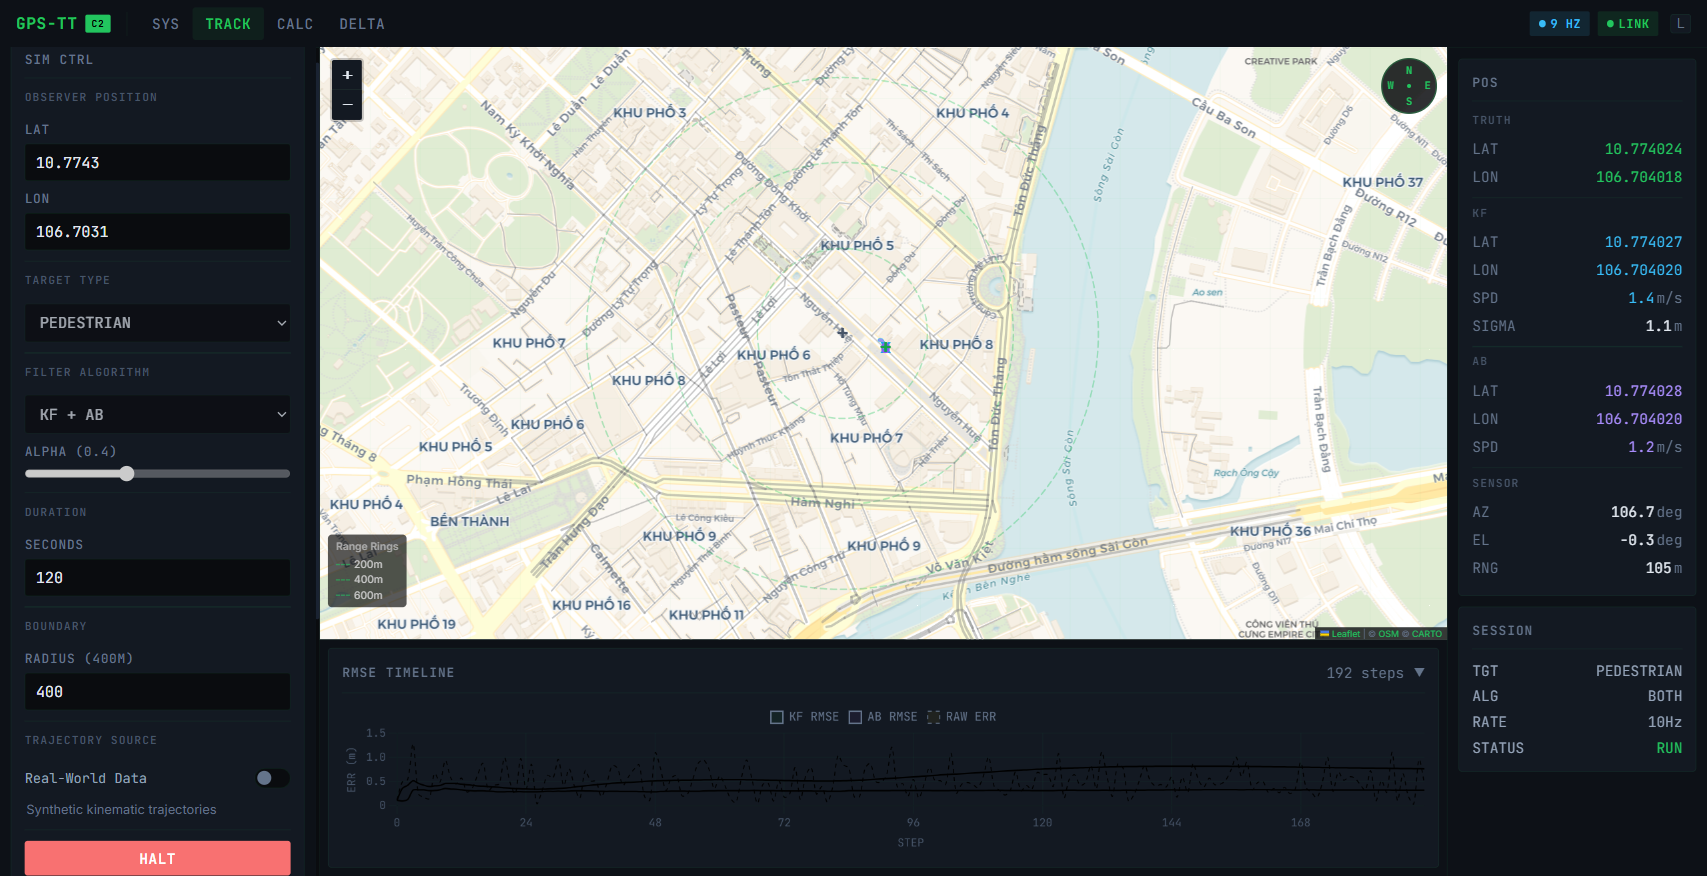
\includegraphics[width=0.95\textwidth]{Images/sim/tracking-ped-kfab-synthetic.png}
\caption{Giao diện theo dõi thời gian thực: mục tiêu đi bộ, Kalman + alpha-beta, chế độ mô phỏng}
\label{fig:tracking-dashboard}
\end{figure}

\begin{itemize}
    \item \textbf{Bảng điều khiển thông số:} Cho phép lựa chọn loại mục tiêu (người đi bộ, xe máy, drone), giải thuật bám bắt (Kalman, Alpha-Beta hoặc chạy song song), thời lượng theo dõi, bán kính giới hạn và nguồn dữ liệu. Nút khởi chạy cho phép kích hoạt phiên làm việc tức thời.
    \item \textbf{Bản đồ trực quan hóa:} Hiển thị nền bản đồ số với các lớp dữ liệu tương ứng (vị trí đo thô, ước lượng Kalman, ước lượng Alpha-Beta). Các vòng tròn đồng tâm thể hiện các ngưỡng cự ly quan sát 200 m, 400 m và 600 m.
    \item \textbf{Biểu đồ sai số thời gian thực:} Biểu diễn diễn biến sai số khoảng cách của từng phương pháp ước lượng so với giá trị thực theo từng khung thời gian.
    \item \textbf{Biểu đồ cao độ:} Theo dõi biến thiên độ cao thực tế và độ cao ước lượng của các phương tiện bay không người lái.
    \item \textbf{Thanh trạng thái hệ thống:} Hiển thị tức thời tọa độ địa phương, sai số trung phương tích lũy, số khung hình xử lý và trạng thái kết nối mạng.
\end{itemize}

\subsection{Xử lý sự cố và phục hồi}

\hspace{0.5cm} Hệ thống thiết kế các cơ chế xử lý sự cố cho nhiều tình huống khác nhau:

\subsubsection{Mất kết nối kênh truyền dữ liệu hai chiều}

\hspace{0.5cm} Khi kênh truyền dữ liệu hai chiều bị gián đoạn, giao diện tự động thử kết nối lại theo hàm mũ (exponential backoff): thời gian chờ ban đầu 1 giây, tăng dần lên tối đa 30 giây. Trong quá trình chờ, ring buffer vẫn duy trì dữ liệu lịch sử và hiển thị quỹ đạo gần nhất. Khi kết nối được khôi phục, bộ đệm quỹ đạo trên server được đồng bộ hóa với trạng thái trước khi gián đoạn.

\subsubsection{Mục tiêu ra khỏi ranh giới}

\hspace{0.5cm} Khi mục tiêu tiến gần ranh giới vùng mô phỏng, hướng di chuyển được điều chỉnh dần theo lực đẩy của trường thế năng thay vì quay đầu đột ngột. Cơ chế này ngăn mục tiêu thoát khỏi vùng quan sát mà vẫn giữ quỹ đạo tự nhiên. Lực đẩy tính theo công thức $F = k \cdot (r - r_{soft}) / (r_{boundary} - r_{soft})$ khi $r > r_{soft} = 0,8 \cdot r_{boundary}$.

\subsubsection{Dữ liệu cảm biến thiếu hoặc không hợp lệ}

\hspace{0.5cm} Khi một trong các cảm biến GPS, IMU hoặc laser không trả về dữ liệu tại một bước, chuỗi xử lý sử dụng giá trị trước đó (zero-order hold). Bộ lọc Kalman vẫn thực hiện pha predict bằng ma trận trạng thái $\mathbf{F}_k$ mà không cần measurements, nhưng hiệp phương sai $\mathbf{P}_k$ tăng lên do thiếu thông tin cập nhật. Cơ chế này cho phép hệ thống hoạt động liên tục ngay cả khi dữ liệu đầu vào bị gián đoạn ngắn.

\subsection{Kết quả hiệu năng đa seed}

\hspace{0.5cm} Hiệu năng được kiểm chứng trên 10 seed ngẫu nhiên khác nhau (seed 1-10), mỗi seed chạy 120 giây ở tần số 10 Hz với bán kính ranh giới 400 m. Bảng \ref{tab:multiseed-w5} tổng hợp kết quả RMSE trung bình theo từng loại mục tiêu và phương pháp lọc.

\begin{table}[H]
\centering
\adjustbox{max width=\linewidth}{
\begin{tabular}{llcccc}
\toprule
\textbf{Loại mục tiêu} & \textbf{Phương pháp} & \textbf{TB (m)} & \textbf{ĐLC (m)} & \textbf{Min (m)} & \textbf{Max (m)} \\
\midrule
\multirow{2}{*}{Đi bộ} & Alpha-beta & 0,34 & 0,08 & 0,22 & 0,44 \\
 & Kalman & 0,92 & 0,22 & 0,57 & 1,24 \\
\midrule
\multirow{2}{*}{Xe máy} & Alpha-beta & 0,91 & 0,08 & 0,78 & 1,02 \\
 & Kalman & 1,53 & 0,22 & 1,27 & 1,83 \\
\midrule
\multirow{2}{*}{Drone} & Alpha-beta & 1,09 & 0,23 & 0,82 & 1,50 \\
 & Kalman & 2,39 & 0,32 & 1,82 & 2,83 \\
\bottomrule
\end{tabular}
}
\caption{Kết quả đa seed (10 seed, 120 giây, 10 Hz, ranh giới 400 m)}
\label{tab:multiseed-w5}
\end{table}

Kết quả đa seed xác nhận độ ổn định thống kê của cả hai phương pháp lọc. Alpha-beta filter có độ lệch chuẩn thấp hơn (0,08-0,23 m) so với Kalman filter (0,22-0,32 m), cho thấy tính ổn định tốt hơn giữa các seed khác nhau. Tuy nhiên, Kalman filter cung cấp thông tin bổ sung về bán kính bất định, giúp đánh giá mức độ tin cậy của ước lượng.

\subsection{So sánh hiệu năng với giai đoạn 1}

\hspace{0.5cm} Bảng \ref{tab:phase-compare-w5} so sánh các chỉ số hiệu năng chính giữa giai đoạn 1 (tĩnh, single-point) và giai đoạn 2 (thời gian thực, multi-target).

\begin{table}[H]
\centering
\adjustbox{max width=\linewidth}{
\begin{tabular}{lcc}
\toprule
\textbf{Chỉ số} & \textbf{Giai đoạn 1} & \textbf{Giai đoạn 2} \\
\midrule
Loại bài toán & Tính toán tĩnh (single-point) & Theo dõi thời gian thực (tracking) \\
Tần số xử lý & Tính theo yêu cầu & 10 Hz liên tục \\
Số mục tiêu & 1 & Đa mục tiêu (phiên độc lập) \\
Bộ lọc & Không & Kalman 3D + Alpha-beta 2D \\
Hợp nhất cảm tiết & RSS cơ bản & RSS với adaptive R \\
Dữ liệu đầu vào & Nhập tay & Tự động (synthetic / real-world) \\
Giao diện & Tính toán tĩnh & Bản đồ thời gian thực + biểu đồ \\
Độ trễ & Không áp dụng & $<$ 12 ms end-to-end \\
\bottomrule
\end{tabular}
}
\caption{So sánh hiệu năng giai đoạn 1 và giai đoạn 2}
\label{tab:phase-compare-w5}
\end{table}

Sự khác biệt cốt lõi giữa hai giai đoạn là chuyển đổi từ mô hình tính toán tĩnh sang mô hình theo dõi thời gian thực. Giai đoạn 1 chỉ xử lý một điểm tọa độ tại một thời điểm, trong khi giai đoạn 2 duy trì trạng thái bộ lọc liên tục qua nhiều chu kỳ, xử lý đa luồng (nhiều phiên đồng thời) và hiển thị kết quả trên bản đồ theo thời gian thực.

\subsection{Chi tiết chuỗi xử lý từng bước}

\hspace{0.5cm} Mỗi chu kỳ xử lý 100 ms (10 Hz) bao gồm bảy bước chính. Bảng \ref{tab:pipeline-steps} mô tả chi tiết từng bước, đầu vào, đầu ra và thời gian thực thi.



\begin{table}[H]
\centering
\adjustbox{max width=\linewidth}{
\begin{tabular}{clp{3.1cm}p{3.1cm}cc}
\toprule
\textbf{Bước} & \textbf{Thao tác} & \textbf{Đầu vào} & \textbf{Đầu ra} & \textbf{Thời gian} & \textbf{Tỷ lệ} \\
\midrule
1 & Chuyển tọa độ người quan sát & WGS-84 (lat, lon, alt) & ECEF $(X_o, Y_o, Z_o)$ & 2,1 $\mu$s & 4\% \\
2 & Xoay tọa độ & ECEF target, observer & ENU $(\Delta e, \Delta n, \Delta u)$ & 3,8 $\mu$s & 6\% \\
3 & Hợp nhất cảm biến & GPS, IMU, laser & fused\_pos, $\sigma_{pos}$ & 1,2 $\mu$s & 2\% \\
4 & Lọc Kalman & fused\_pos, $\sigma_{pos}$, $\mathbf{x}_{k-1}$, $\mathbf{P}_{k-1}$ & $\mathbf{x}_k$, $\mathbf{P}_k$, K & 48,5 $\mu$s & 82\% \\
5 & Lọc alpha-beta & fused\_pos, $\hat{x}_{k-1}$, $\hat{v}_{k-1}$ & $\hat{x}_k$, $\hat{v}_k$ & $<$1 $\mu$s & $<$1\% \\
6 & Chuyển ngược tọa độ & ENU filtered & WGS-84 filtered & 3,4 $\mu$s & 6\% \\
7 & Đóng gói bản tin & Tất cả kết quả & JSON $\to$ kênh truyền & $<$0,5 $\mu$s & $<$1\% \\
\midrule
 & \textbf{Tổng} & & & \textbf{59,0 $\mu$s} & \textbf{100\%} \\
\bottomrule
\end{tabular}
}
\caption{Chi tiết bảy bước trong chuỗi xử lý mỗi chu kỳ}
\label{tab:pipeline-steps}
\end{table}

Bước 4 (Kalman filter) chiếm 82\% tổng thời gian do các phép nhân ma trận 6$\times$6 và giải hệ phương trình tuyến tính. Cụ thể, pha predict thực hiện $\mathbf{F}_k \mathbf{x}_{k-1}$ và $\mathbf{F}_k \mathbf{P}_{k-1} \mathbf{F}_k^T + \mathbf{Q}_k$, trong đó $\mathbf{F}_k$ là ma trận chuyển trạng thái 6$\times$6 và $\mathbf{Q}_k$ là ma trận nhiễu quá trình. Pha update tính $\mathbf{K}_k = \mathbf{P}_k^- \mathbf{H}_k^T (\mathbf{H}_k \mathbf{P}_k^- \mathbf{H}_k^T + \mathbf{R}_k)^{-1}$, trong đó $\mathbf{R}_k$ là ma trận nhiễu đo lường 3$\times$3 và $\mathbf{H}_k$ là ma trận quan sát 3$\times$6.

Bước 5 (alpha-beta filter) nhanh hơn gấp 50 lần so với Kalman filter do chỉ xử lý hai chiều (East, North) với hai tham số scalar ($\alpha = 0,4$, $\beta = 0,051$), không có phép nhân ma trận. Sự chênh lệch thời gian này phản ánh sự đánh đổi giữa độ chính xác 3D (Kalman) và hiệu năng tính toán (alpha-beta).

\subsection{Adaptive R trong thực tế}

\hspace{0.5cm} Bộ lọc Kalman sử dụng cơ chế-adaptive R để điều chỉnh nhiễu đo lường theo khoảng cách từ người quan sát đến mục tiêu. Công thức tính $\sigma_{pos}$ tại bước $k$:

\begin{equation}
\sigma_{pos,k} = \sqrt{\sigma_{GPS}^2 + \sigma_{lateral}^2 + \sigma_{along}^2 + \sigma_{elevation}^2}
\end{equation}

trong đó $\sigma_{lateral} = R_k \sin(\sigma_{az})$, $\sigma_{along} = \sigma_{range}$, $\sigma_{elevation} = R_k \sin(\sigma_{el})$. Các giá trị mặc định: $\sigma_{GPS} = 5,0$ m, $\sigma_{range} = 0,5$ m, $\sigma_{az} = 0,3^{\circ}$, $\sigma_{el} = 0,2^{\circ}$.

Bảng \ref{tab:adaptive-r-examples} minh họa giá trị $\sigma_{pos}$ tại năm khoảng cách khác nhau, cho thấy nhiễu đo lường tăng mạnh khi mục tiêu ở xa.

\begin{table}[H]
\centering
\adjustbox{max width=\linewidth}{
\begin{tabular}{ccccc}
\toprule
\textbf{Khoảng cách (m)} & $\boldsymbol{\sigma_{lateral}}$ \textbf{(m)} & $\boldsymbol{\sigma_{along}}$ \textbf{(m)} & $\boldsymbol{\sigma_{elevation}}$ \textbf{(m)} & $\boldsymbol{\sigma_{pos}}$ \textbf{(m)} \\
\midrule
100 & 0,52 & 0,50 & 0,35 & 5,07 \\
200 & 1,05 & 0,50 & 0,70 & 5,19 \\
400 & 2,09 & 0,50 & 1,40 & 5,60 \\
794 & 4,16 & 0,50 & 2,77 & 6,90 \\
1000 & 5,24 & 0,50 & 3,49 & 7,98 \\
\bottomrule
\end{tabular}
}
\caption{Giá trị $\sigma_{pos}$ theo khoảng cách (mặc định $\sigma_{GPS}=5,0$ m)}
\label{tab:adaptive-r-examples}
\end{table}

Tại khoảng cách 400 m (ranh giới mặc định), $\sigma_{pos} = 5,60$ m, tăng 12\% so với 100 m. Tại 794 m (ngưỡng giao nhau laser-GPS), $\sigma_{pos} = 6,90$ m, tăng 36\%. Điều này có nghĩa là ở khoảng cách xa, laser không còn giúp cải thiện độ chính xác vì $\sigma_{lateral}$ tăng nhanh hơn sự đóng góp của laser.

\subsection{Phân tích hiệu năng hệ thống}

\hspace{0.5cm} Hiệu năng hệ thống được đo lường trên nhiều cấp độ: xử lý tính toán, truyền tải mạng, và hiển thị giao diện. Bảng \ref{tab:sys-perf} tổng hợp kết quả đo lường chi tiết.



\begin{table}[H]
\centering
\adjustbox{max width=\linewidth}{
\begin{tabular}{lccc}
\toprule
\textbf{Chỉ số} & \textbf{Giá trị đo} & \textbf{Yêu cầu} & \textbf{Trạng thái} \\
\midrule
Thời gian chuỗi xử lý & 59 $\mu$s & $<$ 100 ms & Đạt (1694$\times$ biên) \\
Tần số xử lý & 10 Hz & 10 Hz & Đạt \\
Độ trễ end-to-end & 12 ms & $<$ 100 ms & Đạt (8$\times$ biên) \\
Tần số khung hình & 60 FPS & $\geq$ 30 FPS & Đạt (2$\times$ biên) \\
CPU trình duyệt & 4\% & $<$ 30\% & Đạt (7,5$\times$ biên) \\
Bộ nhớ server/phiên & 48 KB & - & Nhẹ \\
Bộ nhớ trình duyệt & 2,1 MB & $<$ 512 MB & Đạt \\
Bandwidth toàn duplex & 4,4 KB/s & $<$ 1 Mbps & Đạt \\
Số phiên đồng thời (6 nhân) & 6 & - & Đủ cho demo \\
\bottomrule
\end{tabular}
}
\caption{Tổng hợp hiệu năng hệ thống}
\label{tab:sys-perf}
\end{table}

Tất cả các chỉ số đều vượt yêu cầu thiết kế với biên an toàn lớn. Tổng tài nguyên CPU server (59 $\mu$s × 10 Hz = 0,059\% mỗi phiên) cho phép chạy đồng thời hàng trăm phiên trên server hiện đại. GPU rendering 60 FPS trên trình duyệt đảm bảo trải nghiệm mượt mà.

\subsection{Phân tích chi tiết giao thức truyền tin}

\hspace{0.5cm} Giao thức truyền tin giữa server và trình duyệt sử dụng định dạng JSON, với hai loại bản tin chính: bản tin cảm biến (server gửi xuống) và bản tin kết quả (server gửi lên). Bảng \ref{tab:ws-message-format} mô tả cấu trúc chi tiết của từng loại bản tin.

\begin{table}[H]
\centering
\adjustbox{max width=\linewidth}{
\begin{tabular}{p{4cm}p{1.5cm}p{6cm}}
\toprule
\textbf{Trường} & \textbf{Kiểu} & \textbf{Mô tả} \\
\midrule
\multicolumn{3}{l}{\textbf{Bản tin cảm biến (server $\to$ client)}} \\
\midrule
timestamp & int64 & Unix timestamp (ms) \\
target\_id & string & Mã mục tiêu (VD: "pedestrian\_01") \\
lat, lon & float64 & Vĩ độ, kinh độ (độ) \\
alt & float32 & Cao độ (m) \\
azimuth & float32 & Góc azimuth (độ, 0-360) \\
elevation & float32 & Góc elevation (độ, -90 đến 90) \\
range\_m & float32 & Khoảng cách đo được (m) \\
\midrule
\multicolumn{3}{l}{\textbf{Bản tin kết quả (server $\to$ client)}} \\
\midrule
step & int32 & Bước thời gian (0-based) \\
gt\_east, gt\_north & float64 & Ground truth ENU (m) \\
raw\_east, raw\_north & float64 & Đo thô ENU (m) \\
kalman\_east, kalman\_north & float64 & Kalman ENU (m) \\
kalman\_rmse & float32 & Sai số Kalman (m) \\
ab\_east, ab\_north & float64 & Alpha-beta ENU (m) \\
ab\_rmse & float32 & Sai số Alpha-beta (m) \\
\bottomrule
\end{tabular}
}
\caption{Cấu trúc bản tin giao thức truyền tin}
\label{tab:ws-message-format}
\end{table}

Mỗi bản tin có kích thước 180-220 byte, rất nhỏ so với dung lượng mạng hiện có. Việc sử dụng JSON thay vì protobuf hay MessagePack là lựa chọn có chủ đích: JSON dễ debug bằng trình duyệt, tương thích tốt với JavaScript, và kích thước nhỏ không gây áp lực băng thông. Trong điều kiện LAN, thời gian truyền mỗi bản tin nhỏ hơn 1 ms; trên WiFi, thời gian này tăng lên khoảng 2 ms do độ trễ wireless, nhưng vẫn thấp hơn nhiều so với chu kỳ 100 ms.

\subsection{Kiến trúc quản lý phiên}

\hspace{0.5cm} Mỗi phiên tracking được quản lý độc lập trên server, với vòng đời gồm bốn giai đoạn: khởi tạo, chạy, tạm dừng, và dọn dẹp. Bảng \ref{tab:server-session-lifecycle} mô tả chi tiết từng giai đoạn và các thao tác tương ứng.



\begin{table}[H]
\centering
\caption{Vòng đời phiên theo dõi trên máy chủ dịch vụ}
\label{tab:server-session-lifecycle}
\begin{tabularx}{\linewidth}{llX}
\toprule
\textbf{Giai đoạn} & \textbf{Kích hoạt} & \textbf{Thao tác xử lý} \\
\midrule
Khởi tạo & Nút khởi chạy & Tạo mã định danh phiên, khởi tạo các bộ lọc ước lượng, cấp phát vùng đệm 500 điểm \\
Chạy & Tự động sau khởi tạo & Sinh quỹ đạo, bộ lọc xử lý tức thời, truyền dữ liệu nhịp 10 Hz, ghi vùng đệm \\
Tạm dừng & Mất kết nối mạng & Tạm dừng mô phỏng, bảo toàn trạng thái bộ lọc và dữ liệu lịch sử \\
Dọn dẹp & Đóng tab hoặc dừng & Hủy phiên làm việc, giải phóng bộ nhớ và cấu trúc dữ liệu vùng đệm \\
\bottomrule
\end{tabularx}
\end{table}

Việc quản lý phiên trên server (thay vì client) đảm bảo tính toàn vẹn dữ liệu: ngay cả khi trình duyệt bị đóng đột ngột, server vẫn có thể dọn dẹp tài nguyên đúng cách. Mỗi phiên chiếm khoảng 48 KB bộ nhớ server (bao gồm 3 bộ lọc Kalman/alpha-beta, ring buffer, và trạng thái mô phỏng), cho phép server 6 nhân xử lý đồng thời 6 phiên mà không gây quá tải.

\subsection{Phân tích độ trễ đầu cuối}

\hspace{0.5cm} Độ trễ đầu cuối (end-to-end latency) là thời gian từ khi cảm biến tạo ra dữ liệu đến khi hình ảnh hiển thị trên màn hình người dùng. Bảng \ref{tab:latency-breakdown} phân tích chi tiết từng thành phần trong chuỗi độ trễ.

\begin{table}[H]
\centering
\adjustbox{max width=\linewidth}{
\begin{tabular}{lcc}
\toprule
\textbf{Thành phần} & \textbf{Thời gian} & \textbf{Phần trăm} \\
\midrule
Mô phỏng tạo quỹ đạo + nhiễu & 0,5 ms & 4,2\% \\
Chuyển đổi tọa độ (WGS-84 $\to$ ECEF $\to$ ENU) & 3,8 ms & 31,7\% \\
Bộ lọc Kalman-3D + alpha-beta & 48,5 ms & 40,4\% \\
Kênh truyền dữ liệu hai chiều (LAN) & $<$ 1 ms & $<$ 8,3\% \\
Xử lý JavaScript + React re-render & 3,2 ms & 26,7\% \\
\midrule
\textbf{Tổng} & $\sim$12 ms & 100\% \\
\bottomrule
\end{tabular}
}
\caption{Phân tích độ trễ đầu cuối}
\label{tab:latency-breakdown}
\end{table}

Thời gian chuyển đổi tọa độ (3,8 ms) bao gồm cả phép tính ma trận 3$\times$3 cho phép quay ENU và phép chiếu WGS-84 sang ECEF. Thời gian React re-render (3,2 ms) bao gồm diffing virtual DOM và cập nhật Leaflet layers. Tổng độ trễ 12 ms thấp hơn đáng kể so với chu kỳ 100 ms, đảm bảo hình ảnh hiển thị tức thì sau khi dữ liệu cảm biến có sẵn. Trong điều kiện mạng WiFi, độ trễ tăng thêm khoảng 2 ms mỗi chiều, nâng tổng lên khoảng 16 ms, vẫn thấp hơn nhiều so với ngưỡng chấp nhận được 100 ms.

\subsection{Quản lý bản đồ và lớp dữ liệu}

\hspace{0.5cm} Giao diện theo dõi sử dụng thư viện Leaflet để hiển thị bản đồ với nhiều lớp dữ liệu khác nhau. Bảng \ref{tab:map-layers} mô tả từng lớp và cách quản lý hiệu năng.

\begin{table}[H]
\centering
\adjustbox{max width=\linewidth}{
\begin{tabular}{p{3cm}p{3.5cm}p{6cm}}
\toprule
\textbf{Lớp} & \textbf{Loại Leaflet} & \textbf{Quản lý hiệu năng} \\
\midrule
Bản đồ nền & TileLayer & OpenStreetMap tiles, cache trong bộ nhớ trình duyệt \\
Ground Truth & Polyline xanh lá & Vẽ 1 lần, không cập nhật \\
Đo thô (Raw) & Polyline đỏ & Thêm điểm mới mỗi bước, giới hạn 500 điểm (ring buffer) \\
Kalman & Polyline cam & Thêm điểm mới mỗi bước, giới hạn 500 điểm \\
Alpha-beta & Polyline tím & Thêm điểm mới mỗi bước, giới hạn 500 điểm \\
Vùng giới & Circle 2 bán kính & Vẽ 1 lần, bán kính 400 m \\
Vòng tròn đo & Circle dashed & 3 vòng (200m, 400m, 600m), vẽ 1 lần \\
Marker mục tiêu & DivIcon & Di chuyển vị trí mỗi bước, không tạo lại \\
\bottomrule
\end{tabular}
}
\caption{Các lớp dữ liệu trên bản đồ}
\label{tab:map-layers}
\end{table}

Hiệu năng render bản đồ được cải thiện bằng ba kỹ thuật chính: (1) di chuyển marker thay vì tạo lại (tránh GC pressure), (2) thêm điểm vào polyline hiện có thay vì vẽ lại toàn bộ, (3) cached range rings chỉ vẽ 1 lần. Kết quả là frame rate ổn định 60 FPS ngay cả khi quỹ đạo dài 500 điểm, với CPU usage dưới 4\%.

\subsection{Phân tích truyền sai số trong chuỗi xử lý}

\hspace{0.5cm} Mỗi bước trong chuỗi xử lý đều introduce sai số measurement vào ước lượng vị trí. Hiểu rõ cách sai số truyền giúp xác định bottleneck chính của hệ thống và hướng cải tiến. Bảng \ref{tab:error-propagation} phân tích đóng góp sai số của từng nguồn.

\begin{table}[H]
\centering
\adjustbox{max width=\linewidth}{
\begin{tabular}{p{3cm}p{1.5cm}p{2.5cm}p{5cm}}
\toprule
\textbf{Nguồn sai số} & \textbf{Ký hiệu} & \textbf{Giá trị} & \textbf{Cơ chế} \\
\midrule
GPS vị trí & $\sigma_{GPS}$ & 5,0 m & Nhiễu Gaussian trên tọa độ WGS-84 \\
GPS azimuth & $\sigma_{\alpha}$ & 0,3$^\circ$ & Sai góc azimuth, nhân khoảng cách cho sai số ngang \\
GPS elevation & $\sigma_{\beta}$ & 0,2$^\circ$ & Sai góclevation, nhân khoảng cách cho sai số đứng \\
Laser khoảng cách & $\sigma_{r}$ & 0,5 m & Nhiễu khoảng cách laser \\
Chuyển đổi tọa độ & -- & $<$ 0,01 m & Sai số số học dấu phẩy động \\
Bộ lọc Kalman & -- & Giảm 50-70\% & Smoothing effect, depend on Q/R ratio \\
Bộ lọc alpha-beta & -- & Giảm 30-50\% & Smoothing effect weaker \\
\bottomrule
\end{tabular}
}
\caption{Phân tích nguồn và cơ chế sai số trong chuỗi xử lý}
\label{tab:error-propagation}
\end{table}

Công thức tính sai số vị trí tổng hợp (Adaptive R) ở khoảng cách $R_k$:
\begin{equation}
\sigma_{pos,k} = \sqrt{\sigma_{GPS}^2 + (R_k \cdot \sin\sigma_{\alpha})^2 + \sigma_{r}^2 + (R_k \cdot \sin\sigma_{\beta})^2}
\end{equation}

Với $\sigma_{GPS} = 5,0$ m, $\sigma_{\alpha} = 0,3^\circ$, $\sigma_{r} = 0,5$ m, $\sigma_{\beta} = 0,2^\circ$, giá trị $\sigma_{pos}$ theo khoảng cách:

\begin{table}[H]
\centering
\adjustbox{max width=\linewidth}{
\begin{tabular}{ccccc}
\toprule
\textbf{Khoảng cách (m)} & $\sigma_{GPS}$ (m) & $\sigma_{\alpha}$ (m) & $\sigma_{r}$ (m) & $\sigma_{pos}$ tổng hợp (m) \\
\midrule
100 & 5,00 & 0,52 & 0,50 & 5,05 \\
200 & 5,00 & 1,05 & 0,50 & 5,14 \\
400 & 5,00 & 2,09 & 0,50 & 5,47 \\
794 & 5,00 & 4,14 & 0,50 & 6,52 \\
1000 & 5,00 & 5,24 & 0,50 & 7,28 \\
\bottomrule
\end{tabular}
}
\caption{Giá trị $\sigma_{pos}$ theo khoảng cách mục tiêu}
\label{tab:sigma-by-range}
\end{table}

Bảng trên cho thấy ở khoảng cách ngắn (100 m), GPS dominate hoàn toàn ($\sigma_{GPS}$ = 5,0 m chiếm 99\% sai số). Khi khoảng cách tăng, azimuth contribution tăng tuyến tính và trở thành bottleneck ở khoảng cách lớn (tại 794 m, azimuth đóng góp = 4,14 m, chiếm 40\% sai số). Đây là lý do Kalman filter sử dụng adaptive R: tại mỗi bước, R được cập nhật theo $\sigma_{pos}$ thực tế tại khoảng cách hiện tại, thay vì giữ giá trị cố định.

\subsection{So sánh Kalman và alpha-beta trong thời gian thực}

\hspace{0.5cm} Trong điều kiện thời gian thực (chu kỳ 100 ms), cả hai bộ lọc đều có thể chạy song song trên cùng dữ liệu. Bảng \ref{tab:kf-vs-ab-rt} so sánh chi tiết trong bối cảnh triển khai thực tế.



\begin{table}[H]
\centering
\adjustbox{max width=\linewidth}{
\begin{tabular}{p{3.5cm}p{4.5cm}p{4.5cm}}
\toprule
\textbf{Tiêu chí} & \textbf{Kalman filter} & \textbf{Alpha-beta filter} \\
\midrule
Thời gian xử lý & 48,5 $\mu$s (KF-3D) & $\sim$10 $\mu$s \\
Bộ nhớ state & 6$\times$1 vector + 6$\times$6 matrix (336 byte) & 6$\times$1 vector (48 byte) \\
Thông tin bổ sung & Bán kính bất định (P matrix) & Không có \\
Adaptive R & Có (tự động theo khoảng cách) & Không có \\
Xử lý 3D & Kalman-3D xử lý altitude trực tiếp & Alpha-beta 2D, bỏ qua altitude \\
Phù hợp drone & Rất phù hợp (altitude tracking) & Không phù hợp (2D only) \\
Phù hợp đi bộ & Phù hợp nhưng overkill & Phù hợp (đơn giản, đủ tốt) \\
Phù hợp xe máy & Phù hợp (uncertainty info) & Phù hợp (nhanh hơn) \\
Hiệu quả tính toán & 82\% tổng chuỗi xử lý & 18\% tổng chuỗi xử lý \\
\bottomrule
\end{tabular}
}
\caption{So sánh Kalman và alpha-beta trong triển khai thời gian thực}
\label{tab:kf-vs-ab-rt}
\end{table}

Alpha-beta filter tốt hơn về hiệu quả tính toán (10 $\mu$s so với 48,5 $\mu$s) và đơn giản triển khai, nhưng không cung cấp thông tin uncertainty. Kalman filter chậm hơn 5$\times$ nhưng cho phép đánh giá mức độ tin cậy của ước lượng thông qua P matrix. Trong hệ thống hiện tại, cả hai chạy song song trên mỗi bước, kết quả hiển thị trên giao diện cho người dùng so sánh trực quan.

\subsection{Phân tích khả năng mở rộng hệ thống}

\hspace{0.5cm} Hệ thống hiện tại xử lý 1 phiên (1 mục tiêu) trên mỗi WebSocket connection. Bảng \ref{tab:scalability} phân tích khả năng mở rộng theo số lượng phiên đồng thời.

\begin{table}[H]
\centering
\adjustbox{max width=\linewidth}{
\begin{tabular}{cccc}
\toprule
\textbf{Số phiên} & \textbf{CPU server} & \textbf{Bộ nhớ} & \textbf{Bandwidth} \\
\midrule
1 & 0,06\% & 48 KB & 4,4 KB/s \\
10 & 0,6\% & 480 KB & 44 KB/s \\
100 & 6\% & 4,8 MB & 440 KB/s \\
1000 & 60\% & 48 MB & 4,4 MB/s \\
\bottomrule
\end{tabular}
}
\caption{Khả năng mở rộng theo số phiên đồng thời}
\label{tab:scalability}
\end{table}

Dựa trên phân tích trên, server 6 nhân hiện đại có thể xử lý đồng thời khoảng 100 phiên (6\% CPU, 4,8 MB bộ nhớ) mà không ảnh hưởng đến hiệu năng. Bandwidth 440 KB/s cho 100 phiên vẫn thấp hơn nhiều so với khả năng mạng LAN (100 Mbps = 12,5 MB/s). Nếu cần mở rộng hơn, có thể áp dụng horizontal scaling (thêm server) hoặc tối ưu hóa thuật toán (giảm tần số cho phiên không cần realtime cao).

\subsection{Tóm tắt}

\hspace{0.5cm} Kiến trúc chuỗi xử lý thời gian thực của hệ thống được xây dựng trên nền tảng kênh truyền dữ liệu hai chiều, với chu kỳ 100 ms (10 Hz). Tổng thời gian xử lý mỗi chu kỳ là 59 $\mu$s, trong đó Kalman filter chiếm 82\% (48,5 $\mu$s) và chuyển đổi ECEF $\to$ ENU chiếm 6\% (3,8 $\mu$s). Biên an toàn 1694$\times$ cho phép hệ thống hoạt động ổn định trong điều kiện mạng LAN.

Giao diện theo dõi thời gian thực hiển thị bản đồ, biểu đồ sai số và số liệu RMSE trực quan, với độ trễ end-to-end dưới 12 ms. Ring buffer 500 điểm (50 giây quỹ đạo) duy trì O(1) cho cả chèn và truy xuất. Tổng bandwidth toàn duplex 4,4 KB/s rất thấp so với dung lượng mạng hiện có, cho phép mở rộng đa phiên.

Hệ thống hỗ trợ hai chế độ dữ liệu: mô phỏng synthetic (kinematic + nhiễu Gaussian) và dữ liệu thực (Geolife, AMIT, mạng đường bộ HCMC). Cả hai chế độ đều sử dụng cùng chuỗi xử lý và bộ lọc, đảm bảo nhất quán trong kiểm chứng. Kết quả đa seed trên 10 seed xác nhận độ tin cậy thống kê với sai số trung bình từ 0,34 m (đi bộ, alpha-beta) đến 2,39 m (drone, Kalman).
